\documentclass{scrreprt}

% allow images
\usepackage{graphicx}
% allow chinese
\usepackage{CJK}
% lists
\usepackage{enumitem}
% hyperlinked TOC (note the CJKbookmarks boolean)
\usepackage[CJKbookmarks = true]{hyperref}
% allow figures and tables to hold position
\usepackage{float}
% pretty tables
\usepackage{booktabs}
\usepackage[table]{xcolor}
% symbols, including \degree for temperatures
\usepackage{gensymb}
% format headers and footers
\usepackage[automark,headsepline,footsepline,plainfootsepline]{scrlayer-scrpage}
\usepackage{csvsimple}
\usepackage{verbatim}
% allow for usage of \Blinddocument to test formatting
\usepackage{mwe}

% options
\graphicspath{{./figures/} {../}}
\definecolor{light-gray}{gray}{0.95}
%% alternate table row colors
\rowcolors{1}{white}{light-gray}

% define macros
\newcommand{\pchapter}[1]{
	\begingroup\let\clearpage\relax
	\newpage
	\begin{figure}[H]
		
\includegraphics[width=0.25\textwidth]{logo.jpeg}
	\end{figure}
	\chapter{#1}
	\endgroup
}
\newcommand{\x}{
	$\times$
}
\newcommand{\ptable}[2]{
	\begin{table}[H]
	\caption{#2}
	\centering\csvautobooktabular{#1}
	\end{table}
}

% define header, title, date
\lohead{
\includegraphics[width=\marginparwidth]{logo.jpeg}}
\title{
	\begin{figure}[H]
		\centering
\includegraphics[width=0.5\textwidth]{logo.jpeg}
	\end{figure}
	\vspace{1cm}
	\flushright
	\Huge{Optical Flow + IMU Module}\\
	\vspace{2cm}
	\huge{First Generation}\\
	\vspace{2cm}
	\LARGE{Prepared by David Qiu \\ on behalf of FRUITION CO., LTD.}
}
\date{
	Last revision: January 18th, 2019\\
}
%%%%%%%%%%%%%%%%%%%%%%%%%%%%%%%%%%%%%%%%%%%%%%%%%%%%%%%%%%%%%%%%%%%%%%%%%%%%%%%%
\begin{document}
\begin{CJK*}{UTF8}{gbsn}
\maketitle
\tableofcontents

\pchapter{Product Overview}

\section{General Description}

Fruition has now released a new low-cost, high-performance, low-latency planar
positioning sensor of optical flowmeter and positioning module. This module
integrates an optical flow tracking sensor, triaxial accelerometer and gyroscope
and one low-power microprocessor.

It can provide positioning information output on surfaces of various materials,
such as tiles, floors, or blankets. Its output is based on the initial
displacement calculated via an internal sensor fusion algorithm relative to
local geographic 3D coordinate bearing data, including the principal axes pitch,
roll, and yaw. The module can also output all sensors' raw data simultaneously.

\section{Applications}

\begin{itemize}
\item Provide orientation information for indoor service robots, such as robot vacuums.
\item Provide positioning information for portable smart toys.
\end{itemize}

\section{Features}

\begin{itemize}
\item Optical tracking and positioning sensor.
\item Adaptable to almost all different indoor surface materials.
\item Adaptable to high velocities, useful in applications utilizing the module for atheltic applications.
\item Small heading sensor, based on MEMS.
\item Integrated high-precision six-axis gyroscope.
\item Stable and accurate sensor fusion algorithm used to calculate the device's displacement.
\item Able to output positioning, orientation, and other information simultaneously.
\item Extremely high stability against ambient temperature and external vibration.
\item UART interface with high baud rate and data output frequency.
\item Low host configuration requirements.
\item Low power consumption.
\end{itemize}

\begin{figure}[H]
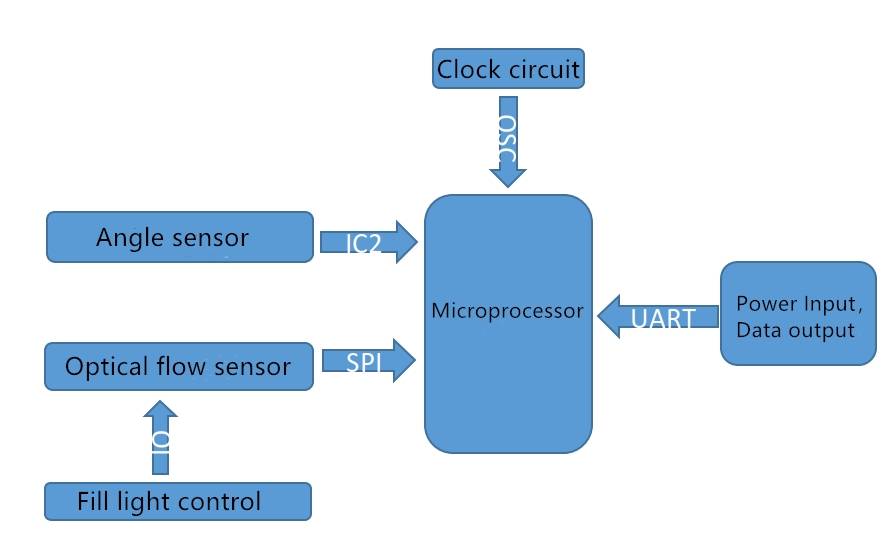
\includegraphics[width = \textwidth]{diagram.png}
\caption{Data flow diagram for the optical flow/IMU module.}
\end{figure}

\pchapter{Detailed Specifications}

\section{Operating Conditions}

\ptable{figures/working_conditions.csv}{%
	The working conditions of the optical flow/IMU module.
}

\ptable{figures/max_rate.csv}{%
	The maximum range of operation conditions of the optical flow/IMU module.
}

\section{Module I/O}

UART configuration is as follows.

\begin{itemize}
\item Baud rate: 115200
\item 8 bit data length
\item Parity NONE
\item 1 bit stop bit.
\item Output frequency is 50 Hz.
\end{itemize}

\ptable{figures/pin_definitions.csv}{%
	The function of the I/O pins on the optical flow/IMU module.
}

\ptable{figures/bit_breakdown.csv}{%
	Data packet format definition on the optical flow/IMU module.
}

\section{Hardware Specifications}

\ptable{figures/detailed_specifications.csv}{%
	Detailed hardware specifications of the optical flow/IMU module.
}

\chapter{Legal}

\textbf{SHENZHEN FRUITION CO., LTD.} shall not be liable, under any
circumstances, for any special, indirect, incidental, consequential, or
contingent damages for any reason, whether or not the buyer has been advised of
the possibility of such damage.

\end{CJK*}
\end{document}
%%%%%%%%%%%%%%%%%%%%%%%%%%%%%%%%%%%%%%%%%%%%%%%%%%%%%%%%%%%%%%%%%%%%%%%%%%%%%%%%
